%% aps to author template--please use pdflatex to edit then to pdf--------------
\documentclass[A4,twoside,fontset=ubuntu,UTF8]{ctexart}
%\usepackage{slashbox}\usepackage{makecell}\usepackage{diagbox}\backslashbox
\usepackage{aappss}
\usepackage{xeCJK}
\usepackage{subcaption}
\usepackage{tabularx}
\usepackage{tikz}

%\usepackage[ruled,vlined]{algorithm}
%\usepackage{algorithmic}
%\floatname{algorithm}{算法}
%\renewcommand{\algorithmicrequire}{\textbf{输入:}}
%\renewcommand{\algorithmicensure}{\textbf{输出:}}
%\usepackage{epstopdf}


\usepackage[linesnumbered,ruled,vlined]{algorithm2e}
\usepackage{setspace}
\usepackage{tcolorbox}
\renewcommand{\algorithmcfname}{算法}
\SetKwInput{KwInput}{输入}
\SetKwInput{KwResult}{输出}
\SetKwComment{Comment}{$\#$\ }{}
\newcommand{\vx}{{\mathbf{x}}}
\def\D{\mathrm{d}}
%\renewcommand\baselinestretch{1.235}\protect
\renewcommand\baselinestretch{2.0}\protect
\newcommand{\bigO}{{\mathcal{O}}}
\newcommand{\ra}[1]{\renewcommand{\arraystretch}{#1}}
\newcommand{\tikzcircle}[2][red,fill=red]{\tikz[baseline=-0.5ex]\draw[#1,radius=#2] (0cm,0.04cm) circle ;}
\definecolor{mygray}{rgb}{0.3333, 0.3333, 0.3333}

\abovedisplayshortskip 0 pt plus 3pt
\belowdisplayshortskip 6 pt plus 2pt minus 2pt
\abovedisplayskip 6 pt plus 2pt minus 2pt
\belowdisplayskip 6 pt plus 2pt minus 2pt
% \info{2015}{64}{1}{01{}} \infodate{2015.0.0.}{2015.0.0.}
%=================== Text begin here ==============================
\begin{document}\apsname

\title{自动微分以及它在物理模拟中的应用\fivestar}%{\cfundlink}

\author{刘金国$^{1)}$ \quad 许开来$^{2)}$}

\address{1)}{哈佛大学物理系, 坎布里奇 \quad 02138}
\address{2)}{斯坦佛大学, 斯坦佛 \quad 94305}

%\address{3)}{}

\abstract{自动微分是利用计算机自动化求导的技术,最近几十年因为它在机器学习研究中的应用而被很多人了解。
如今越来越多的物理学者意识到高效的,自动化的求导可以对很多物理问题的求解提供新的思路。
其中自动微分在物理模拟问题中的应用尤为重要且具有挑战性,其挑战性主要在于如何权衡程序运行的时间与空间。
本文介绍如何将自动微分技术运用到物理模拟的求导中,其中包括共轭态法,前向自动微分,后向自动微分以及可逆计算自动微分等基本方法,
并横向对比了它们在物理模拟中的优势和劣势。}

\keywords{自动微分,科学计算,可逆计算,Treeverse,物理模拟}

% https://ufn.ru/en/pacs/all/
% 02.60.Pn numerical optimization
% 02.30.Jr Partial differential equations
% 91.30.−f Seismology
\pacs{02.60.Pn, 02.30.Jr, 91.30.−f}

\cfund{}

\cmail{jinguoliu@g.harvard.edu \quad }

%\cmailddag{mail2}

%\mail{}{}\cmail \cmailddag

%\apscopyright \baselineskip=16.0pt plus.2pt minus.2pt
%\begin{multicols}{2}\sec
\vskip 0.55\baselineskip
\section{引~~~~言}
    自动微分是指自动获取一段计算机程序导数的技术,很多人对它的了解源自它在机器学习中的成功应用,人们可以用它优化带有千亿计参数的神经元网络~\cite{Rosset2019}。
与很多人印象不同的是,自动微分其实是个很古老的技术。
Nolan早在他1953年的博士论文中就提出过计算机自动化求导的构想~\cite{Nolan1953},
后来针对这一构想又出现了两种不同的实践,分别是1964年由Wengert实现的前向自动微分~\cite{Wengert1964}和1970年Linnainmaa实现的后向自动微分~\cite{Linnainmaa1976}。
而最近十几年,由于后向自动微分在机器学习中的广泛应用,相关技术在科学计算中的应用也越来越广泛。
    %一个典型的例子是变分蒙特卡洛算法。
%过去,人们会将变分基态假设为Gutzwiller波函数~\cite{Gutzwiller1963}这样具有良好解析性质的函数。
%直到2017年,Carleo等人~\cite{Carleo2017, Deng2017}把机器学习中的一些变分模型限制波尔兹曼机(RBM)带入到了大家的视野。由于RBM的解析性质很好,计算所需的求导过程可以通过解析推导,所以当时人们并没有强烈的利用计算机辅助求导的动机。
%但受此启发,大家意识到不光是RBM这样解析性质好的函数,任何机器学习中的神经元网络也可以被用做波函数的猜测形式~\cite{Cai2018}。
%而且如果可以用流行的机器学习框架,比如脸书公司开发的PyTorch和谷歌公司开发的TesnorFlow来编写生成波函数的代码,人们可以避免手动推导导数的麻烦,从而可以把波函数的表达变得更加自由。
%而现在,随着人们对微分的认知更加深刻,波函数不光可以表达为以张量运算为主体的神经元网络,还可以是几乎任意的计算机程序。
科学家们利用方便的,自动化的计算机辅助求导解决了很多重要的物理问题,其中包括变分蒙特卡洛求解多体物理波函数~\cite{Gutzwiller1963,Carleo2017, Deng2017,Cai2018},变分量子算法的模拟~\cite{Luo2019},变分张量网络算法~\cite{Liao2019},以及自旋玻璃基态构型求解~\cite{Liu2020}等。
%甚至是一些非解析的蒙特卡洛抽样过程,人们也设计出了一些办法对其自动化的求导~\cite{Zhang2019}。

本文回顾并探讨自动微分重要应用之一,对物理模拟过程的自动微分。更具体的说是对电磁学,海洋学~\cite{Heimbach2005}和地震学~\cite{Symes2007,Zhu2020}等问题中最核心的微分方程求解过程的自动微分。
这些微分方程的常见的求解方法是将问题的空间部分网格化,从而转换为对时间的常微分方程。
很多现有的包括Jax, PyTorch在内的面向机器学习的自动微分框架中处理后向自动微分对于处理这类问题是棘手的。
因为这些框架需要存储程序每一步计算的信息以便在后向传播过程中取出用于回传梯度。
这对本身内存空间消耗巨大,且计算步骤数很多的物理模拟过程的积分来说并不实际。
之所以说空间开销巨大,是因为要模拟的足够精细,空间网格必须要非常稠密,而步骤数多是为了让对时间的常微分更加准确而要求积分步长足够小。
一种传统的解决自动微分对空间的需求的方案叫做共轭态法~\cite{Plessix2006,Chen2018},它假设了在较短时间内积分器可逆,并通过逆向积分来帮助自动微分回溯状态。
事实上,除了Leap frog等少数积分器在时间反演不变的哈密顿量问题中可以做到时间反演对称,大多数的积分器并不能保证严格可逆,所以共轭态法往往存在由积分步长带来的系统性误差。
后来,有人把机器学习中的最优检查点算法带入到了物理模拟的状态回溯中~\cite{Symes2007},仅在对数的额外时间和空间开销下避免了系统误差。而本文作者也发现与此类似的可逆计算~\cite{}中的Bennett算法也可以用于用利用较少的空间回溯中间状态。本文将会介绍共轭态方法,前向自动微分以及基于最优检查点算法和可逆计算的后向自动微分在处理物理模拟问题中的应用,以及不同方法的优劣。

%那物理学家们是否只需要奉行“拿来主义”,仅阅读机器学习库的文档,就可以很好的驾驭自动微分呢?
%并不完全是的,当大家谈论自动微分的时候有“狭义”和“广义”之分,而主流机器学习库仅涵盖了前者。
%这里狭义自动微分是指机器学习库中广泛应用的以张量为基本数据类型的自动微分。它通过对常用的函数族(矩阵乘法,卷积函数,relu函数等)手动定义导数后向传递的规则,并通过链式法则将它们连接起来得到程序的导数。
%手动定义常用函数导数可以对函数有更加针对性的优化从而保证张量运算的性能,但缺点是,它往往无法满足科学计算的研究中对函数求导的多元化需求。有些时候人们可以通过手动添加一些求导规则来辅助求导,比如在张量网络等模拟中需要用到的复数奇异值分解函数~\cite{Wan2019,Liao2019}。
%但是也有一些时候添加求导规则也无济于事,比如,严格对教化求解基态过程中用到的极大极小本正值求解器~\cite{Xie2020}和模拟变分量子算法中幺正量子线路的求导~\cite{Luo2019}的求导,前者涉及了无法表达为向量函数的稀疏矩阵的构造过程而后者涉及了利用可逆性回溯中间状态。
%还有些时候手动定义的导数可能会出错,尤其是将定义在实数上的规则拓展到复数域的时候。比如奇异值分解函数的求导规则直到2019年,才有人意识到复数的求导规则中有一个规范不变性带来的一项被忽略了~\cite{Wan2019}。
%而广义的自动微分没有这些问题,它微分规则定义在标量的最基础的运算之上,这些基础运算有限而且很难出错。但它在张量运算中的性能却不尽如人意。
%一个很好的描述它与狭义自动微分区别的例子是,当将两个复数相加,广义的自动微分看到的是实部相加和虚部相加这两个操作,而狭义自动微分则需要推导适用于复变函数的Wirtinger导数~\cite{Hirose2003}。

章节\ref{sec:forwardbackward}~ 介绍了共轭态法和自动微分的基本原理。
章节\ref{sec:timespace}~ 介绍了基于检查点和可逆编程的两种后向自动微分的基础理论,尤其两者如何权衡程序的运行时间和空间。
章节\ref{sec:applications}~ 介绍了不同自动微分技术在地震波模拟过程中的应用。

\section{共轭态法与自动微分方法}\label{sec:forwardbackward}

    物理模拟过程的常见求解方案是将偏微分方程的空间部分离散并作差分处理~\cite{Grote2010},将其转换为对时间的常微分方程
    $$\frac{\D s}{\D t} = f(s, t, \theta)$$
其中$s$为状态,$t$为时间,$\theta$为控制参数。假设我们已经拥有一个常微分方程方程求解器来得到末态
这个常微分方程求解器在求解过程中会把时间离散化,作$n$步叠代,每步仅做从时刻$t_i$到时刻$t_{i}+\Delta t$的演化。

\begin{align}
    \begin{split}
    s_n &= \text{ODESolve}(f, s_0, \theta, t_0, t_n)\\
        &= (s_{i+1} = {\rm ODEStep}(f, s_{i}, \theta, t_i, \Delta t) ~\text{for $i=0,2, \ldots, n-1$})
    \end{split}
\end{align}
其中$s_i$为完成第$i$步积分后的状态。
最后我们还会定义一个损失函数$\mathcal{L} = {\rm loss}(s_n)$。
    自动微分的目标则是求解损失量对参数的导数$\frac{\partial \mathcal{L}}{\partial s_0}$, $\frac{\partial \mathcal{L}}{\partial \theta}$, $\frac{\partial \mathcal{L}}{\partial t_0}$和$\frac{\partial \mathcal{L}}{\partial t_n}$。
    %$$s_{i+1} = s_{i} + f(s_i, t, \theta)$$

\subsection{共轭态方法}
    共轭态方法~\cite{Plessix2006,Chen2018}是专门针对积分过程反向传播的传统方法。在研究中,人们发现积分过程的导数的反向传播同样是一个积分过程,只不过方向相反。
    于是人们通过构造一个可以同时更新原函数和导数的拓展函数,以对拓展函数的逆向积分的形式完成导数的计算,如算法~\ref{alg:adjointstate}所示。
\begin{algorithm}
    \setstretch{1.35}
    \SetAlgoLined
    \DontPrintSemicolon
    \SetKwProg{Fn}{function}{}{end}
    \KwInput{动力学参数$\theta$,开始时间$t_0$,结束时间$t_n$,末态$s_n$,以及需要回传的导数$\frac{\partial \mathcal{L}}{\partial s_n}$}
    \KwResult{$\frac{\partial \mathcal{L}}{\partial s_0}$, $\frac{\partial \mathcal{L}}{\partial \theta}$}
        $\frac{\partial \mathcal{L}}{\partial t_n} = \frac{\partial \mathcal{L}}{\partial s_n}^Tf(s_n,t_n,\theta)$ \Comment*[r]{计算损失函数对终了时间的导数}
        \Fn{\rm aug\_dynamics(($s$, $a$, -), $t$, $\theta$) \hspace{14em}$\#$ 定义拓展动力学函数}{$s'=f(s, t, \theta)$ \; \textbf{return} ($s'$, $-a^T\frac{\partial s'}{\partial s}$, $-a^T\frac{\partial s'}{\partial \theta}$)}
        $S_0$ = ($s_n$, $\frac{\partial \mathcal{L}}{\partial s_n}$, $0$) \Comment*[r]{计算拓展动力学函数的初始状态}
        ($s_0$, $\frac{\partial \mathcal{L}}{\partial s_0}$, $\frac{\partial \mathcal{L}}{\partial \theta}$) = ODESolve(aug\_dynamics, $S_0$, $t_n$, $t_0$, $\theta$) \Comment*[r]{对拓展动力学反向积分}
    \caption{共轭态法}\label{alg:adjointstate}
\end{algorithm}

该算法的描述来自文献~\cite{Chen2018},其中可以找到详细的推导过程,这里对原算法中的符号做了替换以方便读者理解。


\subsection{前向自动微分}
    顾名思义,前向自动微分是指向前(指与程序运行方向相同)传播导数。
    \begin{figure}[t]
        \centering
        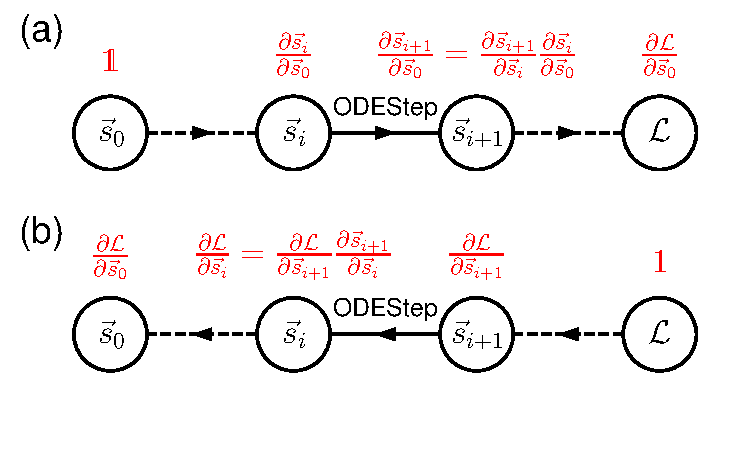
\includegraphics[width=0.7\columnwidth,trim={0 0cm 0 0},clip]{fig3.pdf}

%\begin{subfigure}[b]{0.32\textwidth}
%    \centering
%    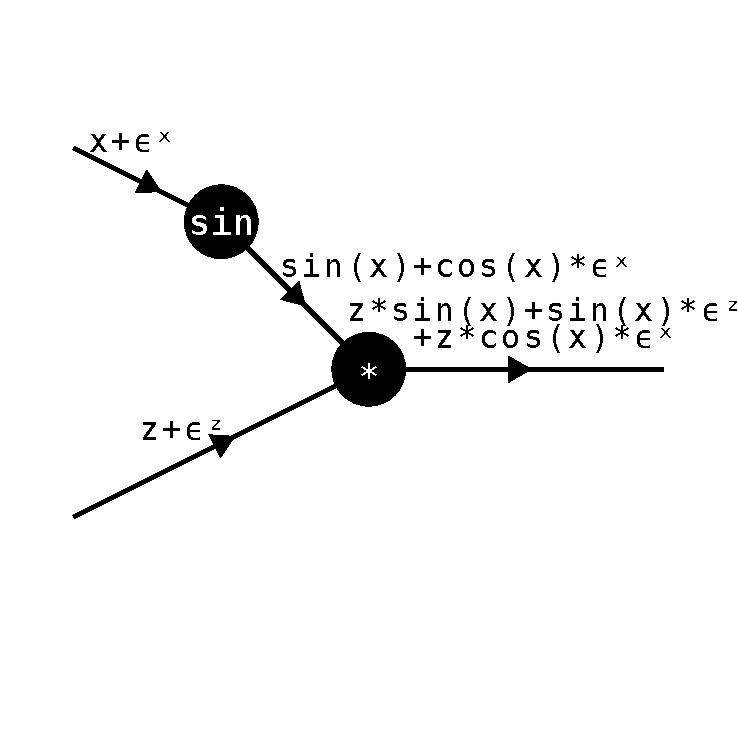
\includegraphics[width=\textwidth, trim={1cm 3cm 0cm 1cm}, clip]{./forwarddiff.pdf}
%    \caption{\small 前向自动微分}
%\end{subfigure}
%\begin{subfigure}[b]{0.32\textwidth}
%    \centering
%    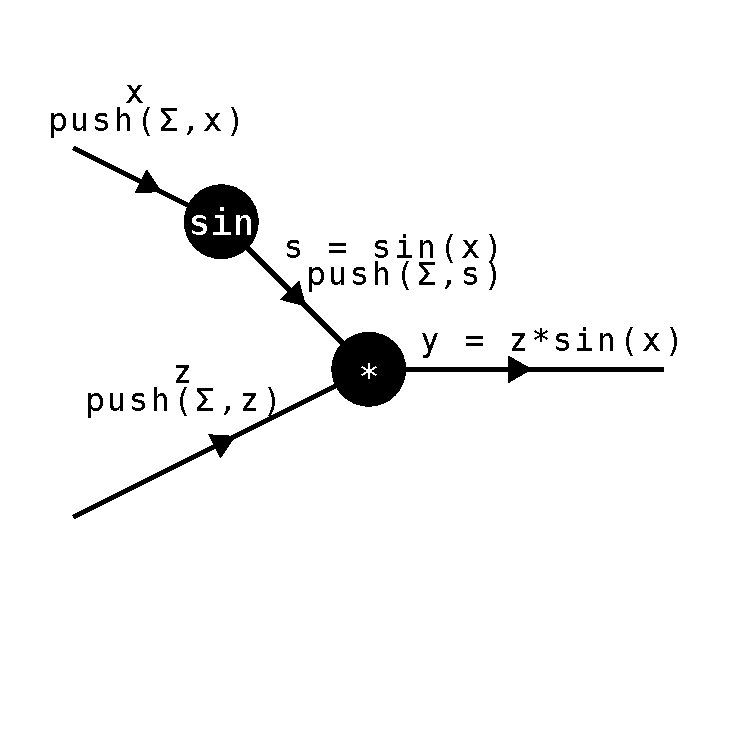
\includegraphics[width=\textwidth, trim={0 3cm 1cm 1cm}, clip]{./backward-forward.pdf}
%    \caption{\small 后向自动微分中的前向计算}
%\end{subfigure}
%\begin{subfigure}[b]{0.32\textwidth}
%    \centering
%    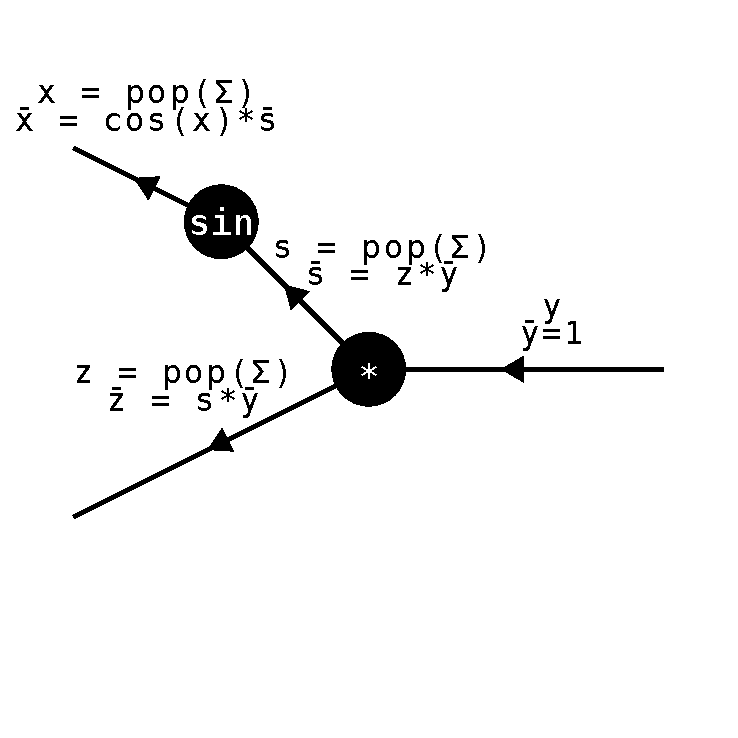
\includegraphics[width=\textwidth, trim={0 3cm 1cm 1cm}, clip]{./backward-backward.pdf}
%    \caption{\small 后向自动微分中的梯度反向传播}
%\end{subfigure}
        \caption{(a) 前向自动微分和 (b) 后向自动微分再常微分方程中的应用,其中圆圈为变量,线条上的箭头梯度传播的方向。}\label{fig:autodifftypes} 
        %\caption{利用自动微分计算对于计算过程$y = z * \sin(x)$的导数$\overline{x}\equiv \frac{\partial y}{\partial x}$和$\overline{z}\equiv \frac{\partial y}{\partial z}$。其中圆圈代表函数,线代表变量,箭头代表运算方向,$\Sigma$是一个用于缓存中间计算结果的全局堆栈(一种以先进后出的存储结构)而\texttt{push}和\texttt{pop}分别代表了对该堆栈的入栈(存储)和出栈(取出)操作。}\label{fig:autodifftypes} 
\end{figure}
数学中,在对一个输入变量$p$求导时,会让它携带一个无穷小量$\D p$,并通过对这个无穷小量的运算完成对程序的求导。比如当作用函数$f$时,会有如下链式法则
\begin{align}
    f(\vec x+ \frac{\D \vec x}{\D p} \D p) = f(\vec x) + \left(\frac{\D f(\vec x)}{\D \vec x}\frac{\D \vec x}{\D p}\right) \D p
\end{align}
其中$\vec x$为输入函数$f$的参数的集合,包括$p$本身。$\frac{\D f(\vec x)}{\D \vec x}$为局域雅可比矩阵,
实际程序实现中,这个局域雅可比矩阵并不需要构造出来。由于任何程序都具有可拆分为基础指令的特点,人们把程序拆解为基础标量指令,并在这些基础指令上实现自动微分的局域变换规则。
具体来说一个标量会同时记录它的数值和一阶小量的系数$(v, \dot v)$,其中$\dot v = \frac{\D v}{\D p}$,人们通过重新定义它的基本运算规则,如
$$\texttt{*}: ((a, \dot a), (b, \dot b)) \mapsto (a * b, a \dot b + b \dot a)$$
使得其在计算同时更新一阶小量的系数。
简单的运算规则的替换对于人类来说尚可手动,但真实的程序可能会包含数以亿计的这样的基础操作,虽然结果依然是解析的,但是人们很难再通过人力得到具体的导数表达式,而计算机恰恰很擅长这样繁琐但是规则简单的任务。
如图~\ref{fig:autodifftypes} (a) 所示,在求解常微分方程中,单步前向自动微分可以形式化的表达为
\begin{align*}
    {\rm ODEStep}^{\rm F} : \left(\left(s_{i+1}, \frac{\D s_{i+1}}{\D s_0}\right), \left(\theta, \frac{\D s_{i+1}}{\D \theta}\right)\right)
        \mapsto &\left(\left({\rm ODEStep}\left(s_{i}, t_i, \theta, \Delta t \right), \frac{\partial s_{i+1}}{\partial s_i} \frac{\D s_{i}}{\D s_0}\right)\right., \\
        &\left.\left(\theta, \frac{\partial s_{i+1}}{\partial s_i} \frac{\D s_{i}}{\D \theta} + \frac{\partial s_{i+1}}{\partial \theta}\right)\right)
\end{align*}
这里为了简洁略去了积分函数和时间等参量。由于状态$s_i, s_{i+1}$和控制参数$\theta$均可包含多个变量,上述偏微分均解释为雅可比行列式。
真实的程序计算中,仅通过基本运算的代码替换或者算符重载即可实现该变换。
%因为一些如\texttt{ForwardDiff}这样优秀的前向自动微分库,我们并不需要手动实现这些链式法则以及基础微分规则。
这里还有一个与计算时间有关的要素,那就是一次对多少个变量求导。如果同时更行整个雅可比行列式,计算空间随着求导变量数目线性增加。
%图~\ref{fig:autodifftypes} (a)所示的是对函数$y=z *\sin(x)$的前向自动微分,这个函数仅仅包含两步运算$\sin$与$*$。程序中每个变量都记录了三个域,分别是\texttt{(变量本身, $\epsilon^x$的系数, $\epsilon^z$的系数)},每当经过一个函数便同时更新数值和两个无穷小量的系数,因此整个函数的运行空间和一次求导的变量的个数也成正比。
在实践中,在内存大小有限且需要求导变量较多的情况下,一般是重复运行多次计算过程,一次只处理若干个变量的导数这样分批次求导。无论是哪种情况,求导时间都会随着需求导的变量的数目线性增长,这是限制前向自动微分应用场景的最主要因素。

\subsection{后向自动微分}
后向自动微分与前向自动微分梯度传播方向相反,它解决了前向自动微分中计算开销随着需要求导的变量数目线性增长的问题。后向自动微分包括前向计算和梯度后向传播两个过程。前向计算过程中,程序进行普通的计算,最后计算得到一个标量为损失$\mathcal{L}$。
梯度回传的过程是计算导数的过程,可表示为更新一个变量的对偶量的过程$\overline{v} = \frac{\partial \mathcal{L}}{\partial v}$。从$\overline{\mathcal L} = 1$出发,
梯度回传即应用如下链式法则
%前向计算过程中除了运算本身,还会将部分运算的中间结果通过\texttt{push($\Sigma$, x)}操作压栈将一个变量\texttt{x}其放入一个全局堆栈$\Sigma$中,
%而后向过程将这些缓存的结果通过\texttt{x = pop($\Sigma$)}操作出栈并利用如下递推公式计算导数
\begin{align*}
    \frac{\D \mathcal{L}}{\D x} &= \sum_y\frac{\partial \mathcal{L}}{\partial y}\frac{\partial y}{\partial x}
\end{align*}
为了实现该链式法则,人们对于一类基础函数$y=f(x)$定义了对偶量的局域运算规则
\begin{align*}
    \overline f: \overline x \mapsto \overline x + \overline y\frac{\partial y}{\partial x}
\end{align*}

其中,$\frac{\partial y}{\partial x}$为局域雅可比矩阵,它的数值不需要具体计算出来,
而是以函数的形式,连同所需的中间变量一起存放在栈中,并在后向传播中按照后进先出的顺序调用。
所有由这一类基础函数构成的代码便可以利用上述导数回传规则更新对偶量。
具体到求解常微分方程的自动微分过程中,其反向传播过程如图~\ref{fig:autodifftypes} (b) 所示,可以形式化的表达为

%\begin{minipage}{0.45\textwidth}
%\begin{align*}
    %{\rm ODEStep}^{\rm B} : s_{i} \mapsto
    %\left(\texttt{push}(\Sigma, s_{i});
    %{\rm ODEStep}(s_{i}, t_i, \theta, \Delta t)\right)
%\end{align*}
%\end{minipage}
%\begin{minipage}{0.45\textwidth}
\begin{align*}
    \overline{\rm ODEStep}^{\rm B} : (\overline s_{i+1}, \overline\theta, s_i) \mapsto %\left(s_{i} = \texttt{pop}(\Sigma);
    \left(\overline{s_{i+1}}\frac{\partial s_{i+1}}{\partial s_{i}}
    ,\overline{\theta} + \overline{s_{i+1}}\frac{\partial s_{i+1}}{\partial \theta}\right)%\right)
\end{align*}
%\end{minipage}
这里也同样略却了积分函数和时间等参量。考虑到该后向传播过程需要知道函数的输入,整个前向计算(左侧)和后向梯度传播(右侧)可表达为

\begin{minipage}{0.45\textwidth}
\begin{align*}
    &\ldots\\
    &\texttt{push}(\Sigma, s_i)\\
    &s_{i+1} = {\rm ODEStep}(s_{i}, t_i, \theta, \Delta t)\\
    &\ldots
\end{align*}
\end{minipage}
\begin{minipage}{0.45\textwidth}
\begin{align*}
    &\ldots\\
    &s_{i} = \texttt{pop}(\Sigma)\\
    &(\overline{s_i}, \overline{\theta}) = \overline{\rm ODEStep}^B(\overline{s_{i+1}}, \overline{\theta},s_i)
    &\ldots
\end{align*}
\end{minipage}

前向计算过程中除了运算本身,还会将部分运算的中间结果通过入栈操作\texttt{push($\Sigma$,$s_i$)}将状态$s_i$的值放入一个全局堆栈$\Sigma$中,而后向过程将这些缓存的结果通过出栈操作\texttt{x = pop($\Sigma$)}取出$s_i$的值并利用后向传播规则更新$\overline s_i$和$\overline \theta$。
%导数回传的计算复杂度与需要求导的变量数目无关,因此它在求导$\sim 10^2$以上的输入变量的优化问题中对比前向自动微分拥有优势,这也是为什么所有的主流自动微分框架都采用梯度后向传播的模式。
%后向自动微分也有缺点,那就是向堆栈中存储数据带来了正比于计算步骤数 ($\bigO(T)$)的额外空间开销以及频繁访问内存带来的性能下降的问题,这是后向自动微分框架设计的复杂性的来源。
虽然导数回传的计算复杂度与需要求导的变量数目无关,但后向自动微分向堆栈中存储数据带来了正比于计算步骤数 (i.e. $\bigO(T)$)的额外空间开销。
如何设计算法在保证对计算状态逆序的访问的前提下,减少计算中使用的堆栈$\Sigma$的大小,是我们在章节~\ref{sec:timespace}中要讨论的一个至关重要的问题。

\section{时间与空间的权衡}\label{sec:timespace}
\subsection{重计算与反计算}
在反向自动微分中,比起将每一步的计算状态保存到堆栈,有时候我们也可以通过“重计算”的方式来得到一部分中间状态。

\begin{minipage}{0.45\textwidth}
\begin{align*}
    &\texttt{push}(\Sigma, s_i)\\
    &s_{i+1} = {\rm ODEStep}(s_{i}, t_i, \theta, \Delta t)\\
    &s_{i+2} = {\rm ODEStep}(s_{i+1}, t_i, \theta, \Delta t)\\
    &\texttt{push}(\Sigma, s_{i+2})
\end{align*}
\end{minipage}
\begin{minipage}{0.45\textwidth}
\begin{align*}
    &s_{i+2} = \texttt{pop}(\Sigma)\\
    %&\overline{s_{i+2}} = \overline{s_{i+3}}\frac{\partial s_{i+3}}{\partial s_{i+2}}\\
    &(\overline{s_{i+2}}, \overline{\theta}) = \overline{\rm ODEStep}^B(\overline{s_{i+3}}, \overline{\theta}, s_{i+2})\\
    &s_{i} = \texttt{read}(\Sigma, \texttt{i})\\
    &s_{i+1} = {\rm ODEStep}(s_{i}, t_i, \theta, \Delta t)  ~\# ~\text{重计算}\\
    %&\overline{s_{i+1}} = \overline{s_{i+2}}\frac{\partial s_{i+2}}{\partial s_{i+1}}\\
    &(\overline{s_{i+1}}, \overline{\theta}) = \overline{\rm ODEStep}^B(\overline{s_{i+2}}, \overline{\theta}, s_{i+1})\\
    &s_{i} = \texttt{pop}(\Sigma)\\
    %&\overline{s_i} = \overline{s_{i+1}}\frac{\partial s_{i+1}}{\partial s_{i}}
    &(\overline{s_i}, \overline{\theta}) = \overline{\rm ODEStep}^B(\overline{s_{i+1}}, \overline{\theta}, s_{i})\\
\end{align*}
\end{minipage}

这里,\texttt{read}函数仅读取数据而不对数据出栈。在正向计算过程中,我们选择性的没有存储状态$s_{i+1}$。
在反向计算过程中,由于状态$s_{i+1}$不存在,程序通过读取$s_{i}$的状态重新计算得到$s_{i+1}$。
通过这种方式,堆栈的大小可以减少1。如何最优的选择存储和释放状态成了检查点方案的关键,
这个最优方案在1992年被Griewank~\cite{Griewank1992}提出,被成为Treeverse算法,该算法仅需对数多个存储空间,即表~\ref{tbl:complexity}所示的空间复杂度$\bigO(S\log(T))$,其中$S$为单个状态的空间大小,$T$为时间,或这里的步数。以及对数的额外时间开销,即时间复杂度$\bigO(T\log(T))$。

还有一种可以保证变量方案叫做可逆编程,意思是让代码在结构上具有可逆性,比如在可逆编程语言的框架下书写代码。
可逆的书写意味着赋值和清除变量这些常见的操作不再被允许,取而代之的是累加 (\texttt{+=}) 和累减 (\texttt{-=}),从内存空“借”一段空内存 ($\leftarrow$) 和将一个已经清除的变量“归还”给内存 ($\rightarrow$)等。
可逆计算赋予用户更高的自由度去控制内存的分配与释放,以如下的程序计算过程(左侧)和它的反过程(右侧)为例

\begin{minipage}{0.45\textwidth}
\begin{align*}
    &s_{i+1} \leftarrow 0\\
    &s_{i+1} \mathrel{+}= {\rm ODEStep}(s_{i}, t_i, \theta, \Delta t)\\
    &s_{i+2} \leftarrow 0\\
    &s_{i+2} \mathrel{+}= {\rm ODEStep}(s_{i+1}, t_i, \theta, \Delta t)\\
    &s_{i+1} \mathrel{-}= {\rm ODEStep}(s_{i}, t_i, \theta, \Delta t) ~\#~\text{反计算}\\
    &s_{i+1} \rightarrow 0 ~\# ~\text{归还}~ s_{i+1}
\end{align*}
\end{minipage}
\begin{minipage}{0.45\textwidth}
\begin{align*}
    &s_{i+1} \leftarrow 0\\
    &s_{i+1} \mathrel{+}= {\rm ODEStep}(s_{i}, t_i, \theta, \Delta t) ~\# ~\text{计算}~ s_{i+1}\\
    &s_{i+2} \mathrel{-}= {\rm ODEStep}(s_{i+1}, t_i, \theta, \Delta t)\\
    &s_{i+2} \rightarrow 0\\
    &s_{i+1} \mathrel{-}= {\rm ODEStep}(s_{i}, t_i, \theta, \Delta t)\\
    &s_{i+1} \rightarrow 0
\end{align*}
\end{minipage}

这里我们先是从状态$s_i$经过两步计算得到了状态$s_{i+1}$和$s_{i+2}$。由于$s_{i+1}$在接下来的运算中不会被用到,我们可以利用已有信息$s_i$将它反计算为$0$,并将存储空间“归还”给系统。
有了反过程,仅需要在反过程中插入求导程序即可完成自动微分。
\begin{align*}
    &(\overline{s_{i+2}}, \overline{\theta}) = \overline{\rm ODEStep}^B(\overline{s_{i+3}}, \overline{\theta}, s_{i+2})\\
    &s_{i+1} \leftarrow 0\\
    &s_{i+1} \mathrel{+}= {\rm ODEStep}(s_{i}, t_i, \theta, \Delta t) ~\# ~\text{计算}~ s_{i+1}\\
    &(\overline{s_{i+1}}, \overline{\theta}) = \overline{\rm ODEStep}^B(\overline{s_{i+2}}, \overline{\theta}, s_{i+1})\\
    &s_{i+2} \mathrel{-}= {\rm ODEStep}(s_{i+1}, t_i, \theta, \Delta t)\\
    &s_{i+2} \rightarrow 0\\
    &s_{i+1} \mathrel{-}= {\rm ODEStep}(s_{i}, t_i, \theta, \Delta t)\\
    &s_{i+1} \rightarrow 0\\
    &(\overline{s_{i}}, \overline{\theta}) = \overline{\rm ODEStep}^B(\overline{s_{i+1}}, \overline{\theta}, s_{i})
\end{align*}
在可逆计算的时间和空间的交换规则下,最优的算法是Bennett算法,其空间的额外开销也是对数,但是时间的额外开销变为了多项式,即表~\ref{tbl:complexity}所示的时间复杂度$\bigO(T^{1+\epsilon})$,其中$\epsilon > 0$,高于最优检查点方案的对数复杂度。
Treeverse算法和Bennett算法分别是源代码后向自动微分(一种通过源代码变换实现的反向传播技术)和可逆计算中权衡时间与空间的核心的算法。为了更好的理解这些算法以方便更好的对物理模拟过程微分,我们用鹅卵石游戏模型来进行说明。

%其实还有一种更加简单的做法是,那就是仅记录程序的初始状态,当需要获取第$k$个计算状态$s_k$,程序从初始状态$s_0$开始进行$k$步运算。这个算法虽然没有额外的空间开销,但是需要$\bigO(T^2)$的运行时间。
%但很多实践中,不管是$\bigO(T^2)$的时间开销或者是$\bigO(T)$的空间开销都不实际,人们更需要的是一个均衡的计算时间和计算空间的方案。
%人们设计出了检查点方案,它的核心思路是在确定在程序运行的何时,何处进行状态拷贝。最优的关于时间和空间交换的检查点方案在1992年被Griewank~\cite{Griewank1992}提出,它是很多广义自动微分框架的基础。
 
%回溯中间状态还有另一种做法,那就是可逆计算。可逆计算的代码不需要借助全局堆栈也可以被回溯。但它并非免费的午餐,因为它也需要额外的空间保证不丢弃信息以保证可逆性。它并不像传统代码一样可以随意的擦除或释放内存,可逆计算“释放”内存的方式是通过反计算把变量内容恢复到0状态,也就是用反计算的时间交换空间。

\subsection{鹅卵石游戏}
鹅卵石游戏是一个定义在一维格子上的单人游戏,它最初被提出描述可逆计算中的时间与空间的交换关系。游戏开始时,玩家拥有一堆鹅卵石以及一个一维排布的$n$个格子,标记为$0,1,2\ldots n$,并且在$0$号格子上有一个预先布置的鹅卵石。
其规则为
\begin{tcolorbox}[width=\textwidth, title=鹅卵石游戏-可逆计算版本]
    \setstretch{1.5}
    \textit{放置规则}:如果第$i$个格子上有鹅卵石,则可以从自己堆中取一个鹅卵石放置于第$i+1$个格子中,\\
    \textit{回收规则}:仅当第$i$个格子上有鹅卵石,才可以把第$i+1$个格子上的鹅卵石取下放入自己的堆中,\\
    \textit{结束条件}:第$n$个格子上有鹅卵石。\\
    \textit{游戏目标}:是在固定可使用鹅卵石数目为$S$ (不包括初始鹅卵石) 的前提下,使用尽可能少的步骤数触发游戏结束。
\end{tcolorbox}
这里一个鹅卵石代表了一个单位的内存,而放置和取回鹅卵石的过程分别代表了计算和反计算,因此均需要一个步骤数,对应计算中的一个单位的运算时间。
这里对应回收规则中要求前一个格点中存在鹅卵石,对应可逆计算在释放内存时,要求其前置状态存在以保证反计算的可行。
当鹅卵石数目充足 ($S\geq n$),我们用$n$个鹅卵石依次铺至终点格子,此时时间复杂度和空间复杂度均为$\bigO(n)$。最少的鹅卵石数目的玩法则需要用到可逆计算框架下时间和空间最优交换方案Bennett算法。

\begin{algorithm}
    \setstretch{1.35}
    \SetAlgoLined
    \DontPrintSemicolon
    \SetKwProg{Fn}{function}{}{end}
    \KwInput{初始状态集合$S=\{0:s_0\}$, 子分块数目$k$, 分块起点$i=0$, 分块长度$L=n$}
    \KwResult{末态$S[n]$}
    \Fn{\rm bennett($S$, $k$, $i$, $L$)}{
        \eIf{$L = 1$}{
            $S[i+1] \leftarrow 0$\;
            $S[i+1] \mathrel{+}= f_i(S[i])$
        }{
            $l = \lceil \frac L k \rceil$\;
            $k' = \lceil \frac L l \rceil$\;
            \For{$j=1,2,...,k'$}{
                bennett($S$, $k$, $i+(j-1)l$, $\min(\frac L k, L-(j-1)l)$) \Comment*[r]{compute k' sub-blocks}
            }
            \For{$j=k'-1,k'-2,...,1$}{
                $\sim$bennett($S$, $k$, $i+\frac{j-1}{k}L$, $\frac L k$) \Comment*[r]{uncompute k'-1 sub-blocks}
            }
        }
    }
    \caption{Bennett算法}\label{alg:bennett}
\end{algorithm}
如算法~\ref{alg:bennett}(图\ref{fig:tradeoff} (b))所示,Bennett算法将格子均匀的分割为$k\geq 2$等份,先是像前执行$k$个区块得到计算结果,然后从最后第$k-1$个区块开始依次收回中间$k-1$个鹅卵石到自由堆中。
每个区块又递归的均匀分割为$k$个子分块做同样的放置鹅卵石-保留最后的鹅卵石-取回鹅卵石的操作,直到程序无法再分割。
假设次过程的递归次数为$l$,我们可以得到步骤数和鹅卵石数为
\begin{align}\label{eq:rev}
    T = (2k-1)^l, S = l(k-1)+1.
\end{align}
其中,$k$与$l$满足$n = k^l$。可以看出可逆计算的时间复杂度和原时间为多项式关系。
同时可以看出$k$ 越小,使用的总鹅卵石数目越小,因此最省空间的鹅卵石游戏解法对应$k=2$。
作为例子,图~\ref{fig:pebbles} (b) 展示了$n=16$,$k=2$ ($l=4$) 时候的游戏解法,对应步骤数为$(T+1)/2 = 41$,这里的实际操作数少了大约一半是因为最外层的Bennett过程不需要取回鹅卵石。

\begin{figure}
    \centerline{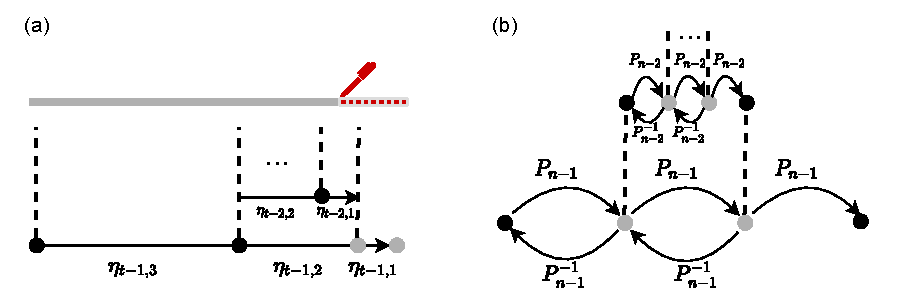
\includegraphics[width=0.88\columnwidth,trim={0 0cm 0 0cm},clip]{tradeoff2.pdf}}
    \caption{(a) 自动微分中常见的Treeverse算法~\cite{Griewank1992},其中$\eta(\tau, \delta) \equiv \left(\begin{matrix} \tau + \delta \\ \delta \end{matrix}\right)=\frac{(\tau+\delta)!}{\tau!\delta!}$。(b) 可逆计算时空交换的Bennett算法。~\cite{Bennett1973,Levine1990} 其中,$P$和$Q$分别代表了计算和反计算。}\label{fig:tradeoff}
\end{figure}


我们稍微修改可以得到非可逆计算的检查点版本的规则。游戏为用户增加了一支画笔用于涂鸦格点,改变后的规则描述为
\begin{tcolorbox}[width=\textwidth, title=鹅卵石游戏-检查点版本]
    \setstretch{1.5}
    \textit{放置规则}:如果第$i$个格子上有鹅卵石,则可以从自己堆中取一个鹅卵石放置于第$i+1$个格子中,\\
    \textit{回收规则}:可以随意把格子上的鹅卵石取下放入自己的堆中,收回鹅卵石不计步骤数,\\
    \textit{涂鸦规则}:当第$i$个格子有鹅卵石,且第$i+1$个格子被涂鸦或$i=n$,可以涂鸦第$i$个格子,涂鸦不记入步骤数,\\
    \textit{结束条件}:涂鸦完所有的格点。\\
    \textit{游戏目标}:是在固定可使用鹅卵石数目为$S$ (不包括初始鹅卵石) 的前提下,使用尽可能少的步骤数触发游戏结束。
\end{tcolorbox}

\begin{figure}
    \centerline{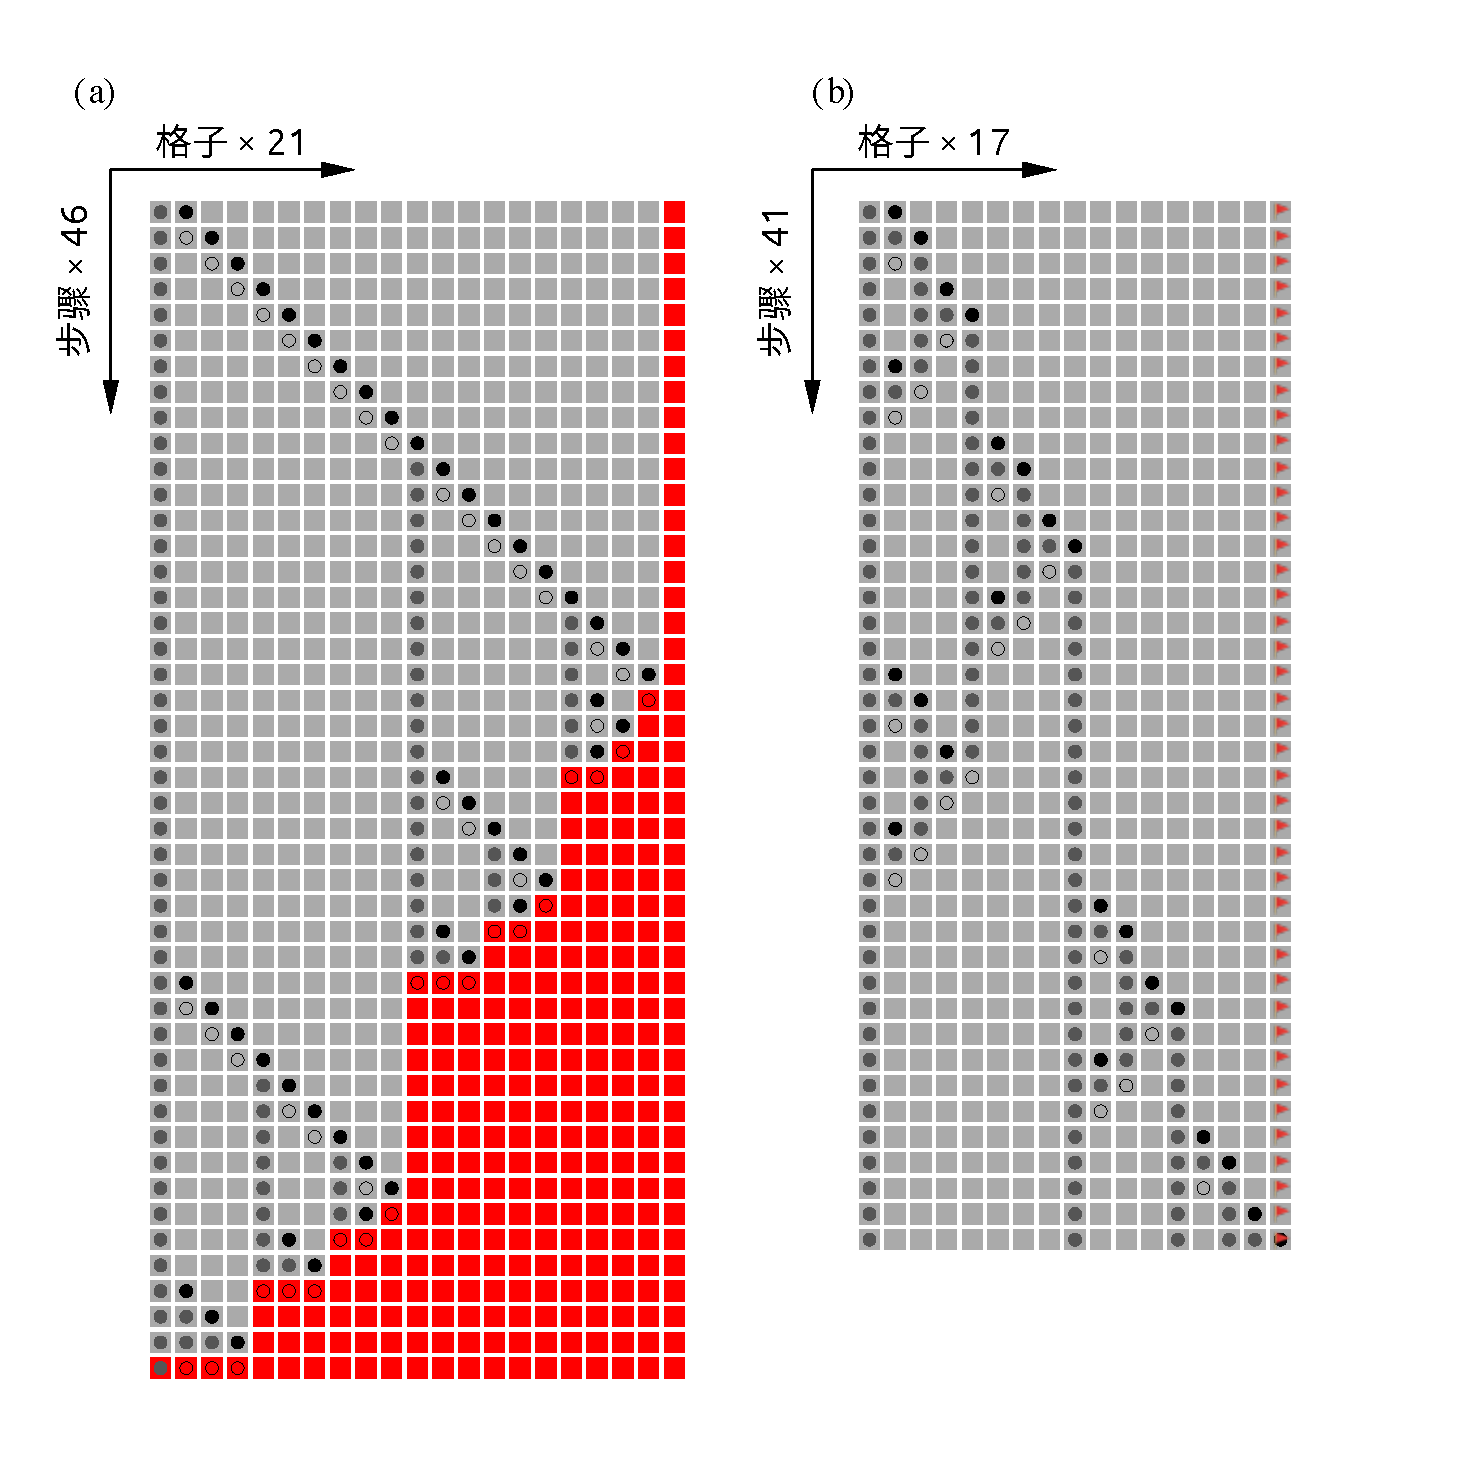
\includegraphics[width=0.88\columnwidth,trim={0 0cm 0 0cm},clip]{bennett_treeverse_pebbles.pdf}}
    \caption{(a) Treeverse算法 ($\tau=3$, $\delta=3$) 和 (b) Bennett算法 ($k=2$, $n=4$) 对应的时间空间交换策略下的鹅卵石游戏,横向是一维棋盘的格子,纵向是步骤。其中“\tikzcircle[black,fill=white]{2pt}”为在这一步中收回的鹅卵石,“\tikzcircle[black,fill=black]{2pt}”为在这一步中放上的鹅卵石,而颜色稍淡的“\tikzcircle[mygray,fill=mygray]{2pt}”则对应遗留在棋盘上未收回的鹅卵石。红色格子代表已被涂鸦,带旗帜的格点代表终点。}\label{fig:pebbles}
\end{figure}

\begin{algorithm}
    \setstretch{1.35}
    \SetAlgoLined
    \DontPrintSemicolon
    \SetKwProg{Fn}{function}{}{end}
    \KwInput{状态缓存集合$S=\{0:s_0\}$,需回传的梯度$\overline{s_n}\equiv \frac{\partial \mathcal{L}}{\partial s_n}$, 允许缓存的状态数$\delta$, 扫描次数$\tau$, 分块起点$\beta=0$,分开终点$\phi=n$,以及把分块分割为两部分的分割点$\sigma=0$}
    \KwResult{回传的梯度$\overline{s_0} \equiv \frac{\partial \mathcal{L}}{\partial s_0}$}
    \Fn{\rm treeverse($S$, $\overline{s_\phi}$, $\delta$, $\tau$, $\beta$, $\sigma$, $\phi$)}{
        \If{\rm $\sigma > \beta$}{
            $\delta = \delta - 1$\;
            %$S[\beta] = s_\beta$   \Comment*[r]{缓存状态 $s_\beta$至状态集合$S$}
            $s = S[\beta]$   \Comment*[r]{加载初始状态 $s_\beta$}
            \For{$j=\beta,\beta+1, ..., \sigma-1$}{
                $s_{j+1} = f_j(s_j)$ \Comment*[r]{计算$s_\sigma$}
            }
            $S[\sigma] = s_\sigma$
        }

         \#~以$\kappa$为最优分割点(二项分布),递归调用Treeverse算法\;
        \While{\rm $\tau>0$ {\bf and} $\kappa={\rm mid}(\delta, \tau, \sigma, \phi) < \phi$}{
            $\overline{s_{\kappa}}$ = treeverse($S$, $\overline{s_\phi}$, $\delta$, $\tau$, $\sigma$, $\kappa$, $\phi$)\;
            $\tau = \tau-1$\;
            $\phi = \kappa$
        }

        $\overline{s_\sigma} = \overline{f_\sigma}(\overline{s_{\sigma+1}}, s_\sigma)$\Comment*[r]{利用已有的$s_\sigma$和$\overline{s_\phi}$回传导数}
        \If{\rm $\sigma>\beta$}{
            remove($S[\beta]$) \Comment*[r]{从缓存的状态集合中移除$s_\beta$}
        }
        {\bf return} $\overline{s_\sigma}$
    }
    \Fn{\rm mid($\delta$, $\tau$, $\sigma$, $\phi$) \hspace{7cm}\# 选取二项分布分割点}{
        $\kappa = \lceil(\delta\sigma + \tau\phi)/(\tau+\delta)\rceil$\;
        \If{$\kappa \geq \phi$ {\bf and} $\delta > 0$}{
            $\kappa$ = max($\sigma+1$, $\phi-1$)
        }
    }
    \caption{Treeverse算法}\label{alg:treeverse}
\end{algorithm}

检查点版本的鹅卵石游戏中,鹅卵石可以被随时取下,代表了传统计算中内存的释放。涂鸦过程则代表了梯度反向传播的过程,它要求按照逆序访问计算状态。在鹅卵石充足的情况下,最节省步骤数的解法和可逆计算版本一样,即计算过程中不取下任何鹅卵石。而用最少鹅卵石的解法则仅需要两枚鹅卵石。每当我们需要涂鸦一个格子$i$,我们总是从初始鹅卵石$s_0$开始扫描(依次放置一个鹅卵石并取下前一个鹅卵石)$i$步至格子$i$,步骤数为$\frac{n(n-1)}{2}$。
鹅卵石数目为$2<\delta<n$的情况最难,需要用到如算法~\ref{alg:treeverse} (图\ref{fig:tradeoff} (a))所示的Treeverse算法。
完成第一遍从$s_0$到$s_{n}$的扫描后会在棋盘上留下$\delta=S-1$个鹅卵石(不包括初始鹅卵石),把格点分割成$\delta$个区块。我们把这些没有被取下的鹅卵石称为检查点,我们总可以从任意一个检查点出发通过放置一个鹅卵石并取回上个鹅卵石的操作扫描后方的格子。
区块的大小有最优的取值为二项分布函数$\eta(\tau-1, \delta), \ldots, \eta(\tau-1, 2), \eta(\tau-1, 1)$,其中$\tau$的取值满足$\eta(\tau, \delta) = n$。
拥有状态$s_{n}$后,$n$号格子直接满足涂鸦规则,因此我们可以在第一遍扫描时给它涂上颜色。
为了继续涂鸦$n-1$号格点,我们从离$n-1$号格点最近的检查点出发扫描至该点,依次类推直至达到最后一个检查点处。
由于最后一个区块尺寸最小,仅为$\tau-1$,我们并不担心这样的扫描会使得步骤数增加太多。
当我们完成了最后一个区块的涂鸦,我们便可把格子上用于标记最后一个区块起点的鹅卵石取下以便重复利用。
为了涂鸦倒数第二个区块,我们先是扫描整个区间,并把这个区间用回收的鹅卵石分割为大小分别是$\eta(\tau-2, 2)$和$\eta(\tau-2, 1)$的两个子区间。
用同样的方式计算最后一个区间并递归的分割前一个子区间直至区块大小为1而无法继续分割。
整个算法的步骤数和鹅卵石数目的关系是
\begin{align}
    T \approx \tau n, S = (\delta+1),
\end{align}
由二项分布的性质可得,$\tau$和$\delta$的大小可以都是$\propto\log(n)$。图~\ref{fig:pebbles} (a) 展示了如何使用Treeverse算法仅用4个鹅卵石,步骤数46涂鸦完所有20个格子。\footnote{这里的46步并不是严格的最优解,因为图中扫描过程的最后一步并不需要立即释放内存从而可以减少步骤数。}

\begin{figure}[h]
\centering
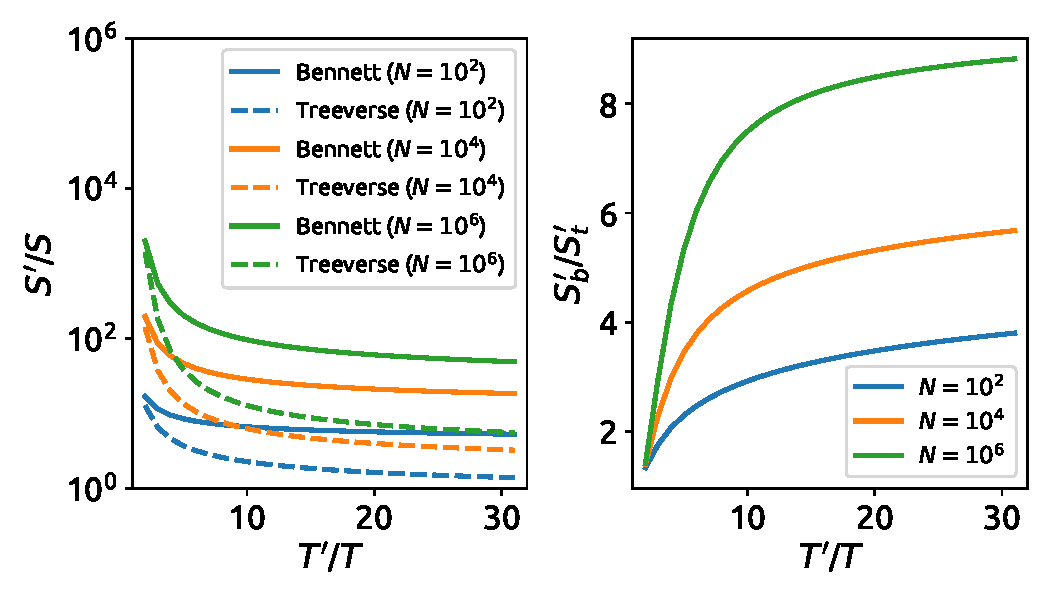
\includegraphics[width=0.8\columnwidth]{./fig1.pdf}
    \caption{为了回溯中间状态,时间和空间在两种最优时间-空间交换策略下的关系。(a) 固定横轴为状态回溯的计算时间与原函数计算时间的比值,对比再允许固定时间开销下,内存的额外开销。其中Bennett算法代表了可逆计算下的最优策略,而Treeverse则是传统计算允许的最优策略,黄色点状横线对应$S'/S=50$。(b) 对比Bennett算法与Treeverse算法空间开销的比值。\label{fig:timespace}} 
\end{figure}

%\begin{figure}
%    \centerline{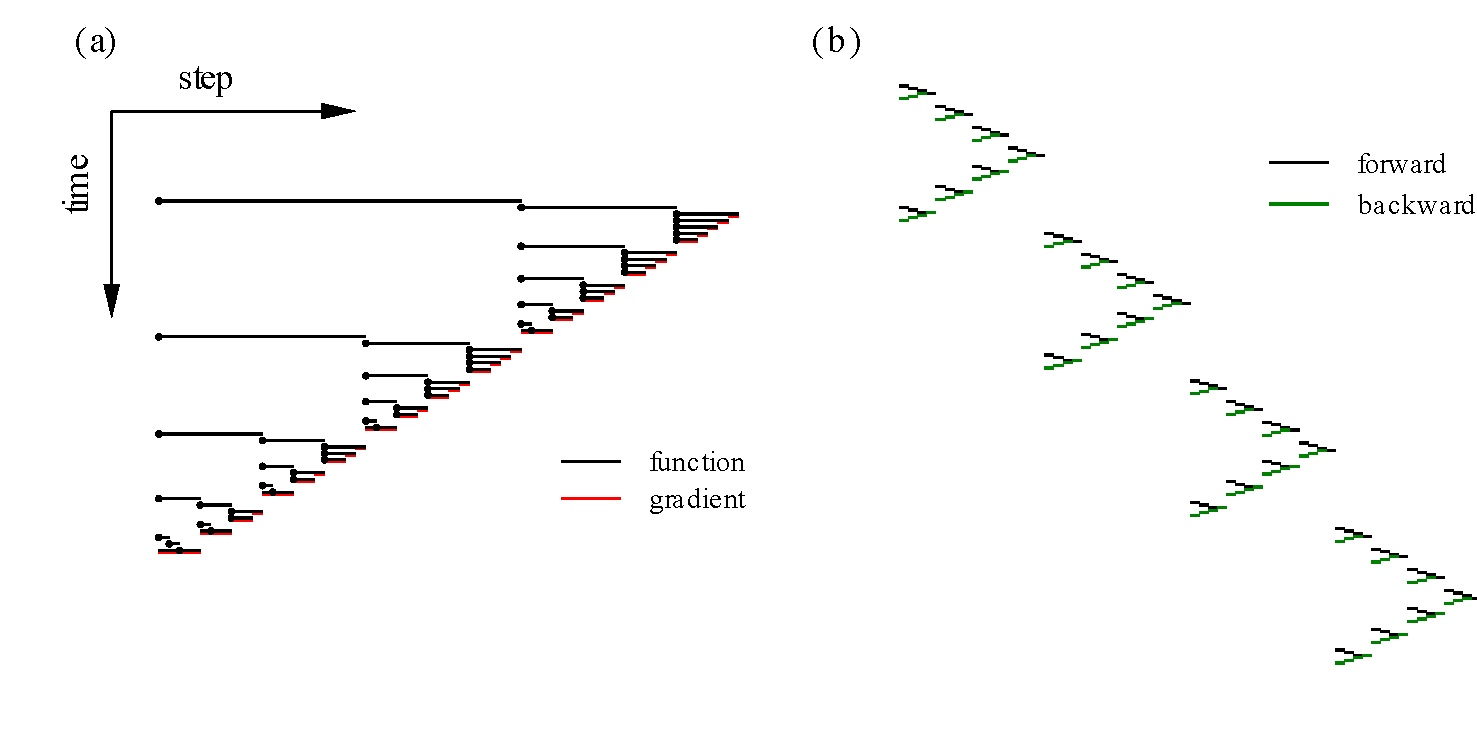
\includegraphics[width=0.88\columnwidth,trim={0 0cm 0 0cm},clip]{bennett_treeverse_fingerprint.pdf}}
%    \caption{(a) Treeverse算法 ($t=5$, $d=3$) 和 (b) Bennett算法 ($k=4$, $n=3$) 中,函数的执行过程,其中横向是鹅卵石游戏的格子,纵向随着进入Treeverse函数或者Bennett函数的次数向下延展。}\label{fig:tradeoff}
%\end{figure}

鹅卵石游戏是对程序的时间和空间的交换关系非常理想化的模型,它恰巧非常合适用于描述常微分方程求解这样不可逆的线性程序。
图~\ref{fig:timespace} 展示了在固定额外时间开销下,程序应用Bennett算法和Treeverse算法得到的最优的空间开销。
可以看出,可逆计算整体上需要更多的空间开销。尤其是当步骤数更多,或是允许的时间的额外开销更大的时候,该差别更加明显。
当程序具有一定结构,可逆计算也有不错的优点,较为直接的优点是可以利用可逆性节省内存。另外由于没有全局堆栈以及对程序自动设置检查点的问题,程序内存管理也更加可控。尤其对于写运行在GPU设备上的可微分函数,避免全局堆栈操作是必要的。

\begin{table}\centering
    \begin{tabularx}{0.7\textwidth}{Xcc}\toprule
        \textbf{方法} & 时间 & 空间\\
        \hline
        共轭态法                     &  $\bigO(T)$          & $\bigO(TS)$\\
        前向自动微分                 &  $\bigO(NT)$         & $\bigO(S)$  \\
        基于检查点的后向自动微分     &  $\bigO(T\log T)$    & $\bigO(S\log T)$   \\
        基于可逆计算的后向自动微分   &  $\bigO(T^{1+\epsilon})$ & $\bigO(S\log T)$ \\
        \bottomrule
    \end{tabularx}
    \caption{不同方案的时间与空间复杂度。其中共轭态法考虑了缓存部分中间结果以保证反向积分的正确性,因此空间会有与时间线性增长。前向自动微分中的$N$代表了需要求导的参数个数。可逆计算中的时间复杂度为多项式,且$\epsilon > 0$。}\label{tbl:complexity}
\end{table}

\section{自动微分在物理模拟中的应用}\label{sec:applications}
本章节有两个案例,其一是用前向自动微分和共轭态法求解参数较少的洛伦茨函数的导数,
其二是用最基于最优检查点算法和Bennett算法的后向微分对参数较多且内存吃紧的地震学模拟的求导。

\subsection{洛伦茨方程求解}
洛伦茨系统是人们研究混沌的经典模型,它描述了一个三维空间中一个坐标点$(x,y,z)$的动力学。该动力学满足洛伦茨方程
\begin{align*}
    \frac{\D x}{\D t} &= \sigma(y - x),\\
    \frac{\D y}{\D t} &= x(\rho -z) - y,\\
    \frac{\D z}{\D t} &= xy-\beta z.
\end{align*}
其中,$\sigma$, $\rho$和$\beta$为三个控制参数,理论上,当$\rho < \sigma \frac{\sigma + \beta + 3}{\sigma - \beta - 1}$时,系统处于稳定状态。数值模拟中,我们用Runge-Kutta方法对时间部分积分并得到末了位置,我们固定初始位置$(x_0,y_0,z_0) = (1, 0, 0)$以及控制参数$\beta=8/3$,积分时间区间为$[0,T=30]$,积分步长为$3\times 10^{-3}$。
末了位置坐标对控制参数和初始坐标的导数反映了末态对控制参数和初始位置的敏感度,它一定程度的反映了浑沌现象。
我们可以用前向自动微分求出终了$x$坐标对初始位置和控制参数的导数$(\frac{\partial x_T}{\partial x_0}, \frac{\partial x_T}{\partial y_0}, \frac{\partial x_T}{\partial z_0})$和$(\frac{\partial x_T}{\partial\sigma}, \frac{\partial x_T}{\partial\rho}, \frac{\partial x_T}{\partial\beta})$的绝对值的平均,并把它们与初始$\rho,\sigma$的关系画在图~\ref{fig:chaos}中。可以看出处于稳定区间(黑线下方)的导数远小于混沌区间(黑线上方)的导数,分界点和理论预言基本一致。

\begin{figure}[t]
\centering
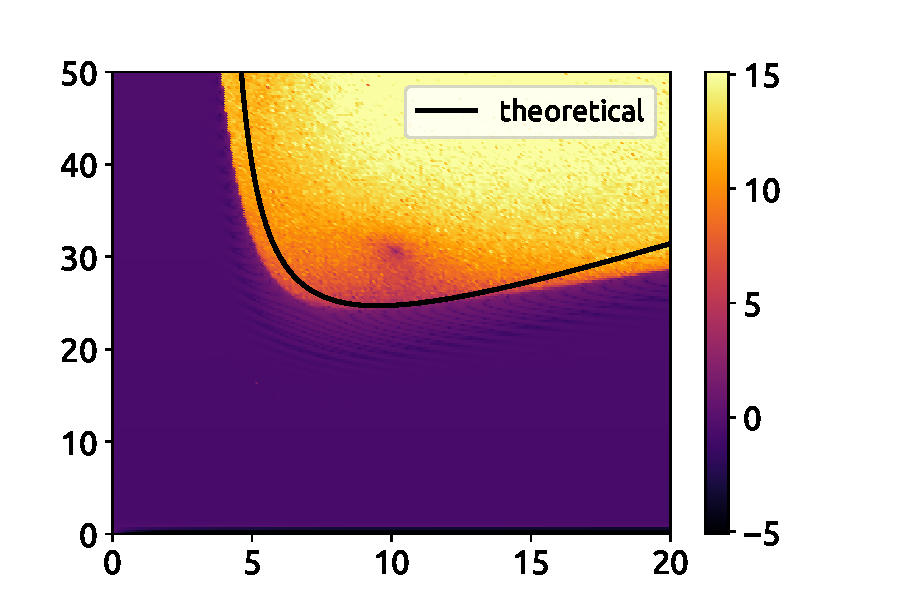
\includegraphics[width=0.6\columnwidth]{./fig4.pdf}
    \caption{Lorenz系统的初始位置和控制参数的导数的大小与系统出现混沌的关系。\label{fig:chaos}} 
\end{figure}

由于这里的参数较少,所以前向自动微分可以做到几乎没有额外时间和空间开销的严格求导。
共轭态法求导理论上也可以做到无额外内存消耗,但是会引入由于积分器不可逆带来的系统误差。我们以前向自动微分的导数是严格的导数作为基准,把共轭态法求得的导数的$l^2$相对误差与积分步长的关系绘制于图~\ref{fig:neuralode-error} (a)中,相对误差随着积分步长指数增加。
因此,我们需要每隔一段积分,就设置一个检查点重新加载严格的导数。图 (b) 显示检查点越密,误差越小,消耗的额外空间也越多。检查点越稀疏,则误差越大,消耗的额外空间越少。

\begin{figure}[t]
\centering
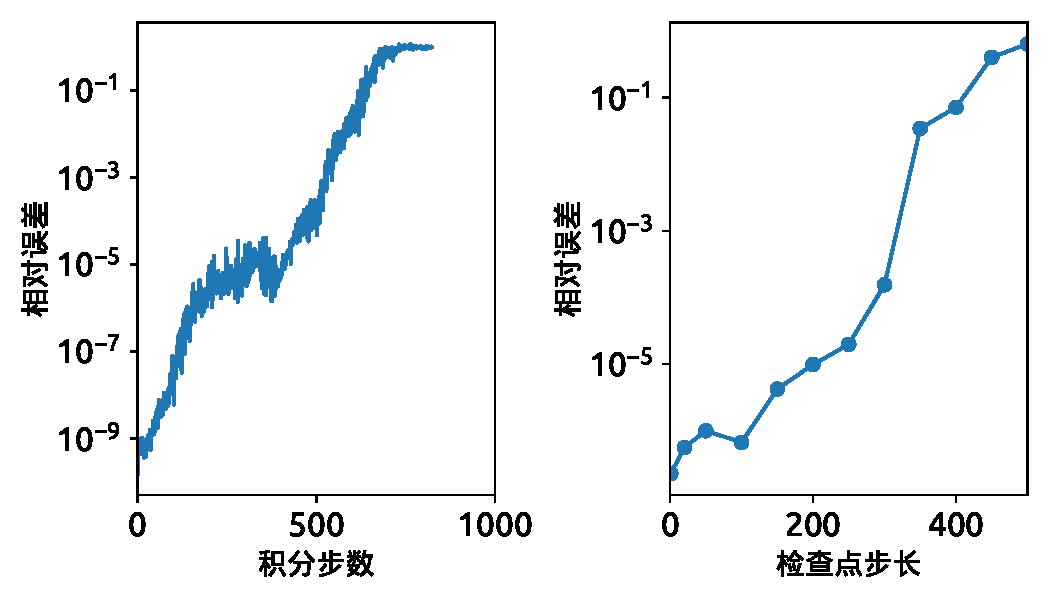
\includegraphics[width=0.6\columnwidth]{./fig2.pdf}
    \caption{利用共轭态方法求导时,$l^2$误差与积分步长的关系。其中一个点代表了在该步长下,对$100$个随机初始点计算得到的中位数。缺失的数据代表该处出现数值溢出的情况。\label{fig:neuralode-error}} 
\end{figure}


\vskip 1.55\baselineskip
\subsection{地震波的模拟}
Perfectly matched layer (PML)方程是模拟波在无限大介质中运动的一种准确可靠的方案,
在介质中,波场$u(\vec x, t)$的传播可描述为
\begin{align}
    \begin{cases}
    u_{tt} - \nabla\cdot(c^2\nabla u) = f & t>0,\\
    u = u_0 & t=0,\\
    u_t = v_0 & t=0.
    \end{cases}
\end{align}
经过对空间的离散化处理
后来在地震学的模拟中,它被用来微分地震波传播的过程~\cite{Symes2007}。
自动微分也在其中发挥着重要的作用~\cite{Zhu2020}。
~\cite{Grote2010}

\begin{figure}[t]
\centering
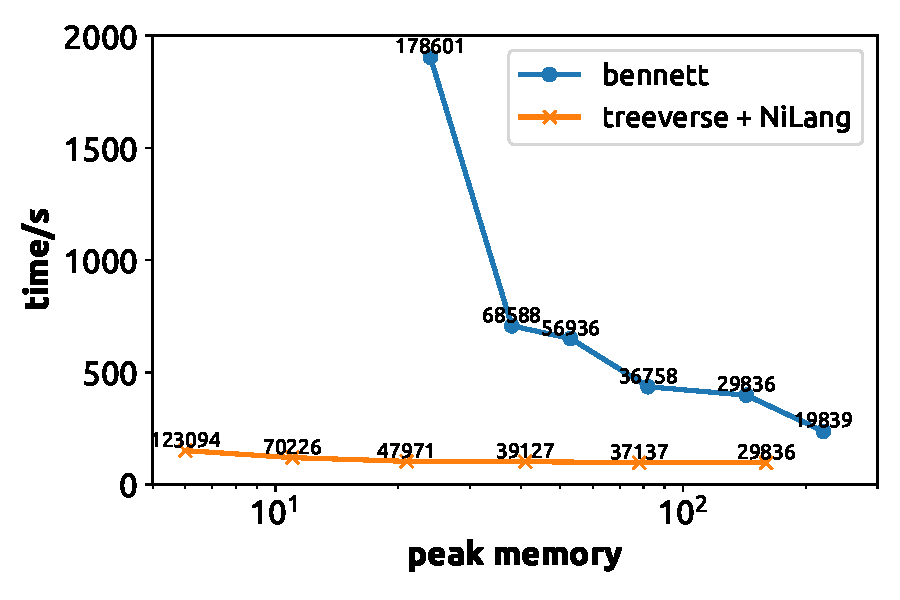
\includegraphics[width=0.6\columnwidth]{./fig5.pdf}
    \caption{对比纯可逆计算的Bennett算法的时间和空间开销和Treeverse算法结合可逆计算的性能,其中图中标记的数字为函数的前向运行次数,在Bennett算法中,后向运行次数和前向运行次数一样,而Treeverse算法中,后向次数固定为$10^4$。\label{fig:seismic}} 
\end{figure}

%\vskip 1.55\baselineskip
%\subsection{热带(Tropical)张量网络求解自旋玻璃最优构型}
%热带张量网络是张量网络的一个特别的应用,它重新定义了张量中基础元素的代数为
%\begin{eqnarray}
%x \oplus y  = \max(x, y),\,\,\,\,\,\,\,\,\,\,\,\, \,\,\,\,
%x \odot y   =  x + y. \label{eq:max-sum-alg}
%\end{eqnarray}
%\begin{figure}[t]
%\centering
%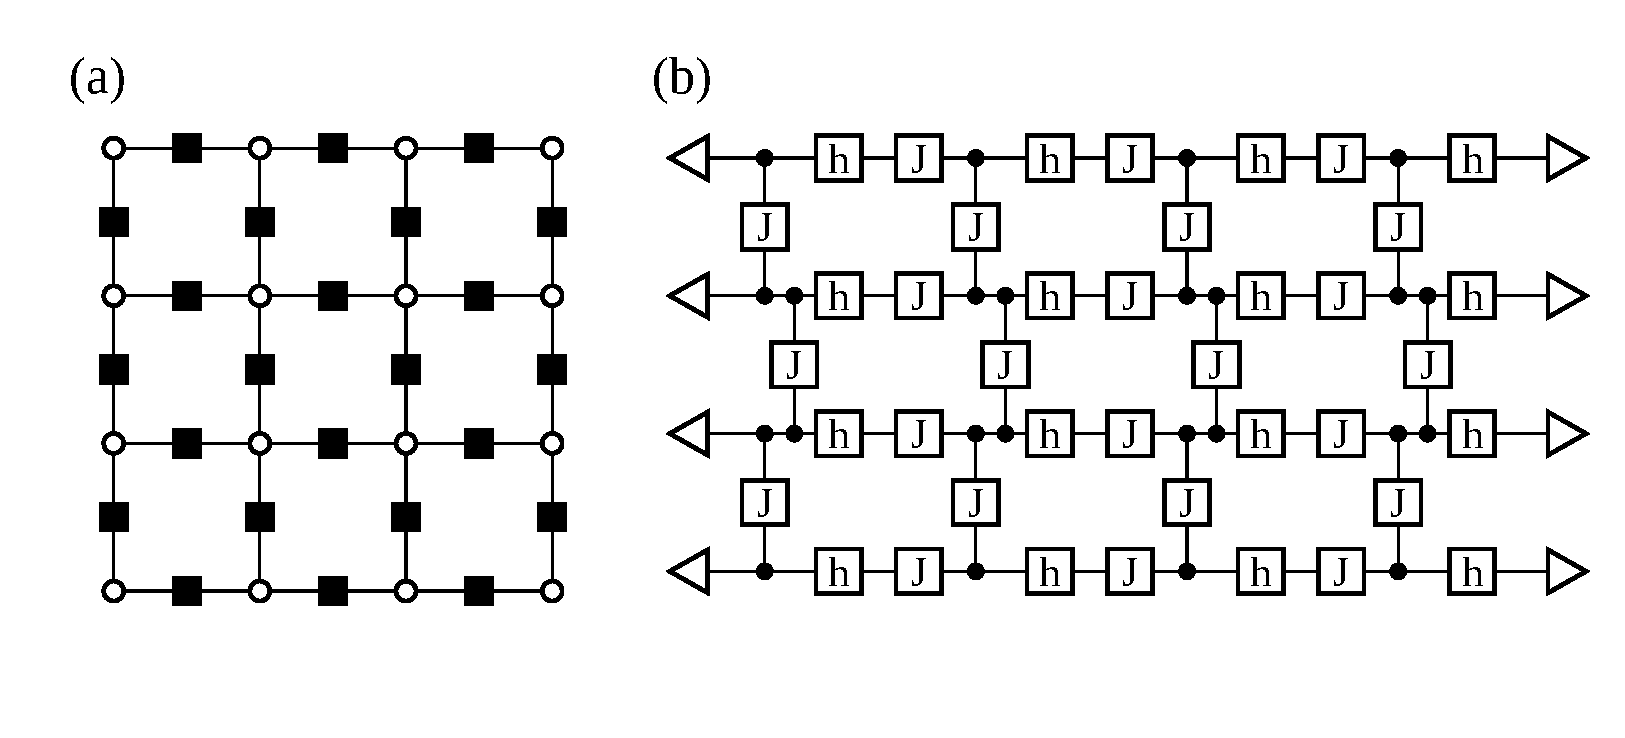
\includegraphics[width=\columnwidth]{./transform12.pdf}
    %\caption{正方晶格上的自旋玻璃问题,(a)对应的热带张量网络表示。(b)对应的“量子线路”表示。\label{fig:performance}} 
%\end{figure}
%如果我们将张量中的元素定义为自旋玻璃的耦合强度,我们就可以通过收缩这个张量结构得到自旋玻璃的最优构型。
%这个最优构型的能量表达式为
%\begin{equation}
    %E(\{\sigma\}) = \max\limits_{\sigma}-\sum_{i < j }J_{ij} \sigma_i \sigma_j  - \sum_i h_i \sigma_i,
%\label{eq:spinglassopt}
%\end{equation}
    %因此对它的微分就是。
%但是作了这样的替换,张量收缩的微分规则就发生了变换。

\section*{致谢}

感谢王磊老师的讨论。
感谢彩云天气CTO苑明理老师的讨论。


\section*{附录A1}

标题排列和编号方式为A1, A2, A3.

\section*{附录A2}
%
%text text
%
%\section*{附录B1}
%%\section*{附录B2}
%
%text text
%
%\section*{致谢}
%
%text text

\bigskip
%\begin{footnotesize}

\bibliographystyle{apsrev4-1}
\bibliography{refs}

\newpage

\title{Automatic differention in physics simulation $^{\ast}$}%{\efundlink}

\efund{Project supported by the State Key Development Program for Basic Research of China (Grant No. 2011CB00000), the National Natural Science Foundation of China (Grant Nos. 123456, 567890), and the National High Technology Research and Development Program of China (Grant No. 2011AA06Z000). \\}



\author{Jin-Guo Liu$^{1)}$ \quad Kai-Lai Xu$^{2)}$}

\address{1)}{Harvard University, Cambridge \quad 02138}
\address{2)}{Stanford University, Stanford \quad 94305}

\email{jinguoliu@g.harvard.edu}
%\email \emailddag

\eaddress{1)}{Massachusetts Hall, Cambridge, MA 02138}

\eaddress{2)}{450 Serra Mall, Stanford, CA 94305}

\eabstract{}

\small  To determine the probe made of amino acids arranged in a linear chain and joined together by peptide bonds between the carboxyl and amino groups of adjacent amino acid residues. The sequence of amino acids in a protein is defined by a gene and encoded in the genetic code. This can happen either
before the protein is used in the cell, or as part of control mechanisms.

\ekeywords{automatic differentiation, scientific computing, reversible programming, Treeverse, physics simulation}

\epacs{02.60.Pn, 02.30.Jr, 91.30.−f}

\end{document}
